% assignment_1.text - Assignment 1 for Machine Learning class (Spring 2015)
% Chanmann Lim - February 2015

\documentclass[a4paper]{article}

\usepackage[margin=1 in]{geometry}
\usepackage{amsmath}
\usepackage{listings}
\usepackage{graphicx}
\usepackage[T1]{fontenc}
\usepackage{float}

\everymath{\displaystyle}

\begin{document}
\setcounter{page}{8}
% \thispagestyle{empty}
% \pagestyle{empty}

\subsection*{4. }

%
% (1) Plot two histograms
%
\paragraph{(1) } Histogram of the Salman and Seabass lightness ~\\
\begin{figure}[H]
  \centering
    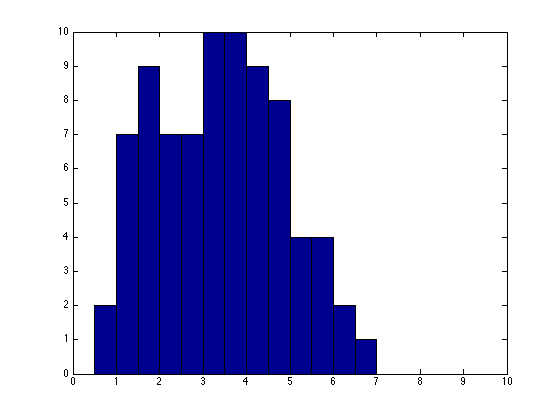
\includegraphics[scale=.6]{images/salmon_hist.png}
  \caption{Salmon lightness histogram}
\end{figure}

\begin{figure}[H]
  \centering
    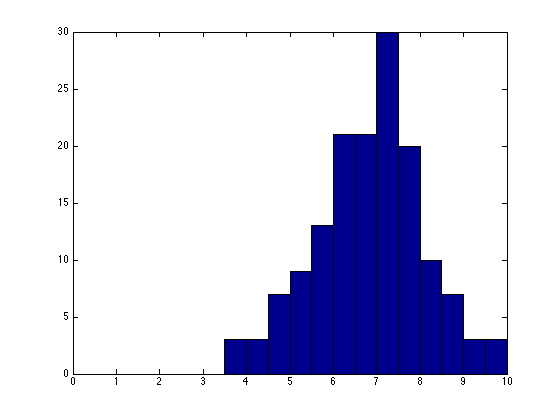
\includegraphics[scale=.6]{images/seabass_hist.png}
  \caption{Seabass lightness histogram}
\end{figure}

%
% (2) Find P(salmon) and P(seabass)
%
\paragraph{(2) } $P(salmon) = 0.34783$ and $P(seabass) = 0.65217$.

%
% (3) Plot P(lightness|salmon) and P(lightness|seabass)
%
\paragraph{(3) } Plots of $P(lightness|salmon)$ and $P(lightness|seabass)$ ~\\

$P(lightness|salmon) = $ [
         0,
    0.0250,
    0.0875,
    0.1125,
    0.0875,
    0.0875,
    0.1250,
    0.1250,
    0.1125,
    0.1000,
    0.0500,
    0.0500,
    0.0250,
    0.0125,
         0,
         0,
         0,
         0,
         0,
         0 ]\\

$P(lightness|seabass)$ = [
         0,
         0,
         0,
         0,
         0,
         0,
         0,
    0.0200,
    0.0200,
    0.0467,
    0.0600,
    0.0867,
    0.1400,
    0.1400,
    0.2000,
    0.1333,
    0.0667,
    0.0467,
    0.0200,
    0.0200 ]
\begin{figure}[H]
  \centering
    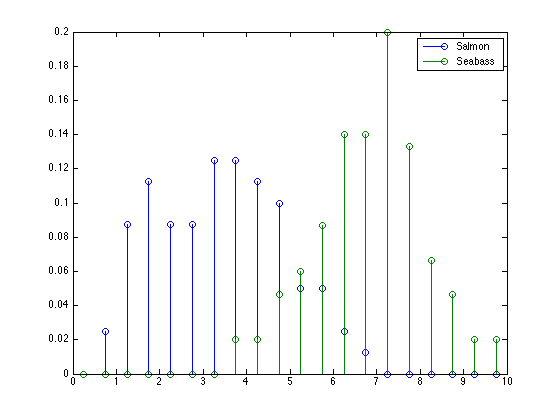
\includegraphics[scale=.6]{images/conditional_probability_pmfs.png}
  \caption{P(lightness|salmon) and P(lightness|Seabass)}
\end{figure}

%
% (4) Compute probabilities
%
\paragraph{(4) } Compute probabilities: ~\\

$P(lightness\le5|salmon) = 0.8625$ and $P(lightness\le8|salmon) = 1$ \\

$P(lightness\ge5|seabass) = 0.91333$ and $P(lightness\ge2|seabass) = 1$

%
% (5) Plot P(lightness)
%
\paragraph{(5) } Plot of the evidence pmf P(lightness) ~\\

$P(lightness)$ = [
         0,
    0.0087,
    0.0304,
    0.0391,
    0.0304,
    0.0304,
    0.0435,
    0.0565,
    0.0522,
    0.0652,
    0.0565,
    0.0739,
    0.1000,
    0.0957,
    0.1304,
    0.0870,
    0.0435,
    0.0304,
    0.0130,
    0.0130 ] \\
\begin{figure}[H]
  \centering
    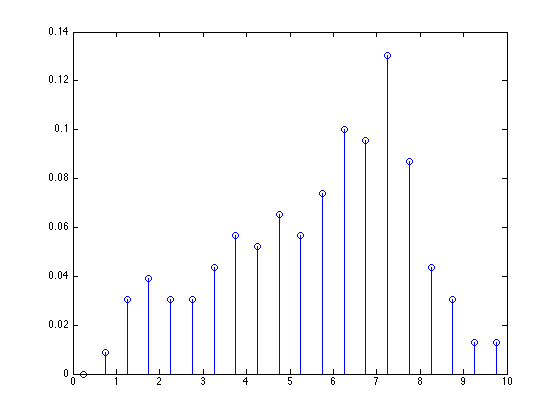
\includegraphics[scale=.6]{images/p_lightness.png}
  \caption{P(lightness)}
\end{figure}

%
% (6) Plot posterior probabilities
%
\paragraph{(6) } Plot the posterior probabilities $P(salmon|lightness)$ and $P(seabass|lightness)$ ~\\

$P(salmon|lightness)$ = [
         0,
    1.0000,
    1.0000,
    1.0000,
    1.0000,
    1.0000,
    1.0000,
    0.7692,
    0.7500,
    0.5333,
    0.3077,
    0.2353,
    0.0870,
    0.0455,
         0,
         0,
         0,
         0,
         0,
         0 ]\\

$P(seabass|lightness)$ = [
         0,
         0,
         0,
         0,
         0,
         0,
         0,
    0.2308,
    0.2500,
    0.4667,
    0.6923,
    0.7647,
    0.9130,
    0.9545,
    1.0000,
    1.0000,
    1.0000,
    1.0000,
    1.0000,
    1.0000 ]

\begin{figure}[H]
  \centering
    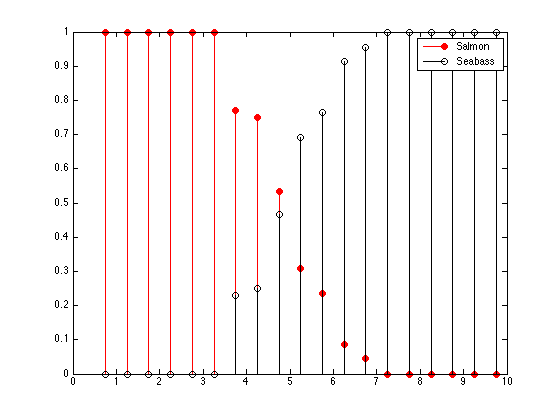
\includegraphics[scale=.6]{images/posterior_probabilities.png}
  \caption{Posterior probabilities}
\end{figure}

\newpage
\subsection*{Appendix:}
\lstinputlisting[language=Matlab, title=\lstname, basicstyle=\footnotesize]{assignment_1.m}

\end{document}